\documentclass[10pt,xcolor=table]{beamer}
 
% \usepackage[utf8]{inputenc}
% \usepackage[T1]{fontenc}
\usepackage[table]{xcolor}    % loads also »colortbl« 
%  \usepackage{enumitem}
\usepackage{ucltemplate}
\usepackage{color}

% \definecolor{parCol}{rgb}{0.1, 0.1, 1}
% \definecolor{stCol}{rgb}{0.1, 0.6, 0.1}
% \definecolor{bothCol}{rgb}{0, 0.5, 0.5}

\definecolor{parCol}{rgb}{0, 0, 0}
\definecolor{stCol}{rgb}{0, 0, 0}
\definecolor{bothCol}{rgb}{0, 0, 0}

\usepackage{graphicx,subcaption}

%Information to be included in the title page:
\title{AAIC Express: Data Sharing Platforms \\(Featured Research Session)}
\author{Razvan Valentin Marinescu}
% \institute{Center for Medical Image Computing, University College London}

% logo of my university

\setbeamersize{text margin left=15pt,text margin right=15pt,text margin bottom=15pt}

\begin{document}
 
\frame{\titlepage}
 
\setbeamerfont{frametitle}{size=\large}

% Worldwide many clinical studies are ongoing on the pathophysiology, diagnosis, prognosis and treatment of Alzheimer’s disease. The potential of these studies is not fully used as they not yet linked to each other. Several data-sharing initiatives have started in recent years. Aim of this Featured Research Symposium is to inform about these initiatives and to stimulate their use for data analysis and selection of subjects for future studies. The symposium will have presentations on 4 initiatives: 1) Dementia Platform United Kingdom (DPUK). This is an integrated dementias research environment that enables rapid analysis of multiple independent data sets.  2) The European Prevention of Alzheimer’s Dementia (EPAD) Registry. The registry aims to provides access to ongoing studies and enables selection of subjects for other studies including trials. 3) The Global Alzheimer's Association Interactive Network (GAAIN). This is a gateway providing access to a vast collection of Alzheimer's disease research data, sophisticated analytical tools, and computational resources. 4) The European Medical Information Framework for Alzheimer’s disease (EMIF-AD). This is a Europe based initiative, which provides a catalogue of on-going studies, pipelines for data harmonisation into a common ontology, and central data-storage.

%DPUK has also invested in scanning equipment(7 PET-MR scanners), 
\begin{frame}
\frametitle{Dementias Platform UK (DPUK)}

\begin{itemize}
% \item Integrated dementias research environment
\item Enables rapid analysis of 38 UK-based existing studies (2 million subjects)
\item Available data: EHRs, genetic, imaging and wearables data
\item Infrastructure investments:
\begin{itemize}
 \item 7 PET-MR scanners
 \item Multi-modal informatics network
 \item Stem-cell network
\end{itemize}
% \item Data must be analysed remotely
\item DPUK goals:
\begin{itemize}
 \item Enables risk stratification for early phase trials
 \item Technology development for 
 \begin{itemize}
 \item molecular and structural imaging
 \item stem cell reserch 
 \item bio-informatics
\end{itemize}
% \vspace{-2em}

\end{itemize}


\end{itemize}


\vspace{-1em}
\begin{figure}
\centering

\includegraphics[height=2.5cm,right]{DPUK_logo}   
\end{figure}
\vspace{-4em}

\end{frame}


\begin{frame}
\frametitle{Dementias Platform UK (DPUK)}


\begin{figure}
\centering
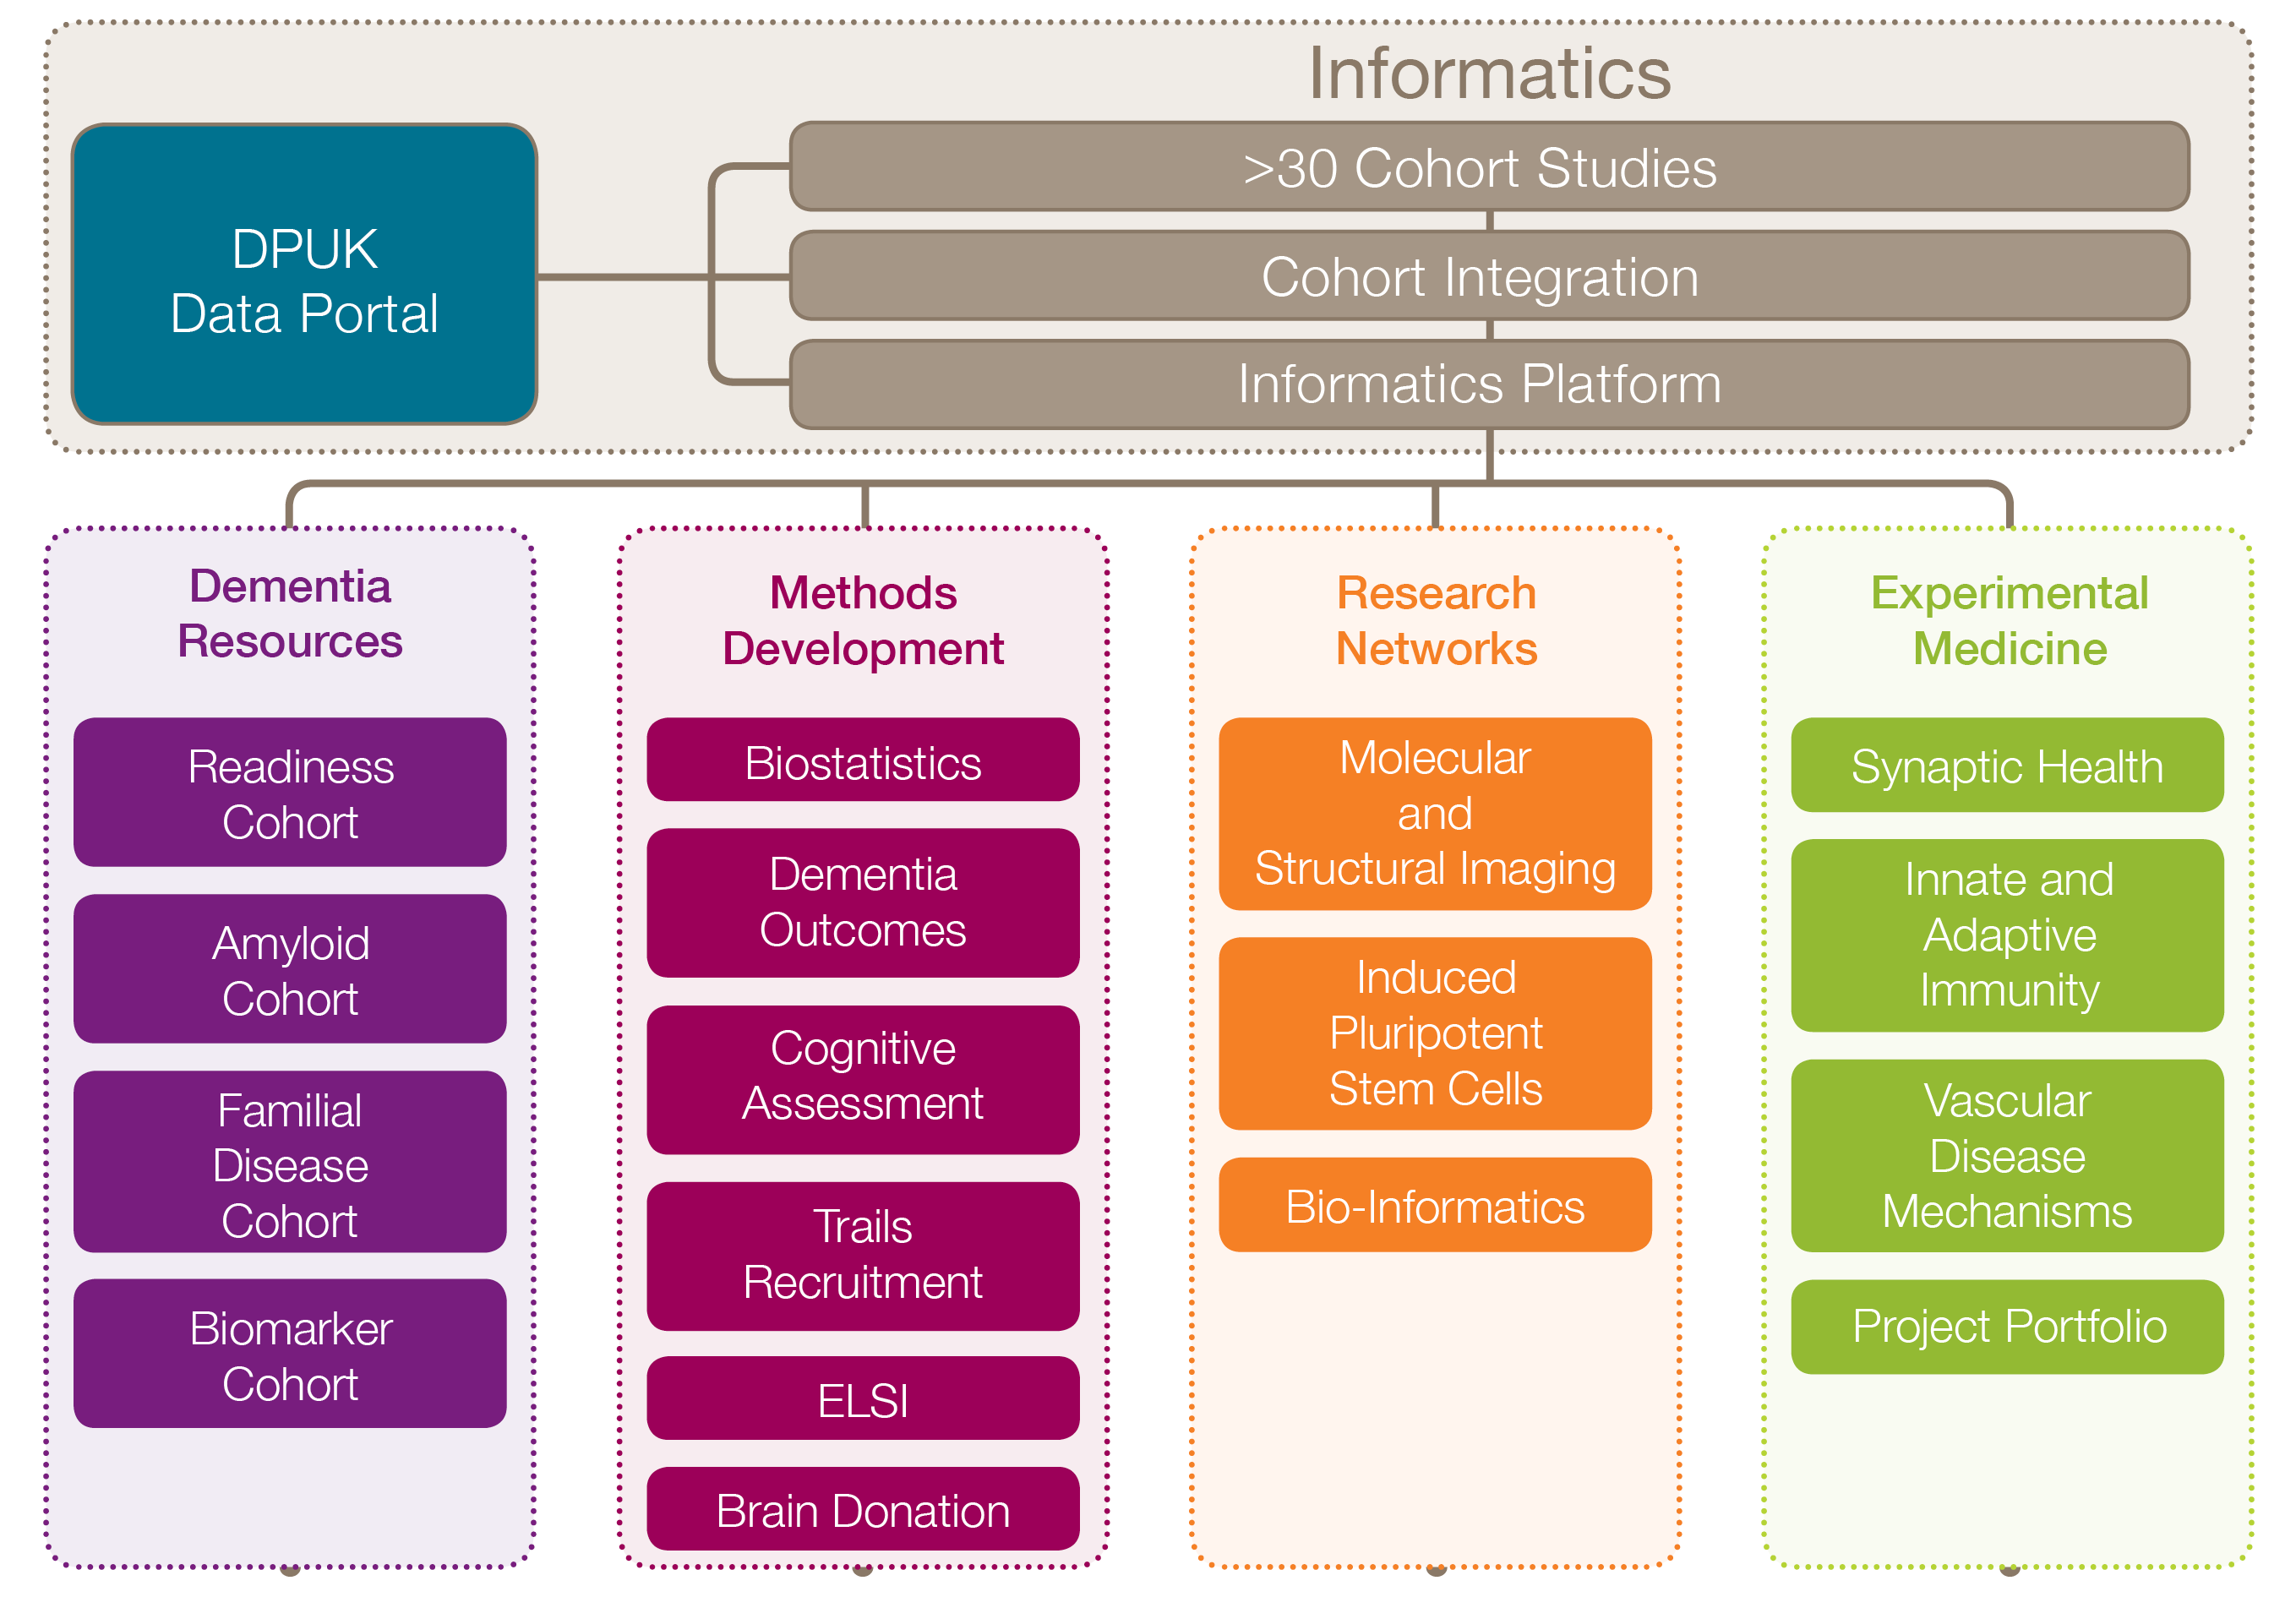
\includegraphics[height=7cm,right]{DPUKdiagram}   
\end{figure}
\vspace{-4em}

\end{frame}

\begin{frame}
\frametitle{European Prevention of Alzheimer’s Dementia (EPAD)}


\includegraphics[height=1.5cm,right]{EPADlogo}  
\vspace{1em}
\begin{itemize}
 \item Recruiting participants for AD trials is difficult
 \item EPAD allows recruitment of suitable patients from other clinical trials
 \item 9 cohorts currently signed up, 17,000 non-demented participants
 \item Cohort owners provide anonymised data on AD risk factors and demographics
 \item Adaptive Clinical trials: 
\end{itemize}

\begin{figure}
% \begin{subfigure}{0.4\textwidth}
% \end{subfigure}\\
\begin{subfigure}{1\textwidth}
\centering
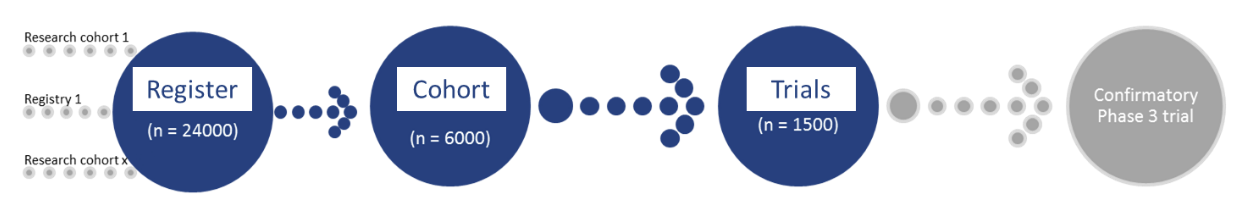
\includegraphics[height=2cm,right]{epad_flow}  
\end{subfigure}
\end{figure}
\vspace{-1em}
\end{frame}

\begin{frame}
\frametitle{Global Alzheimer's Association Interactive Network}

\begin{itemize}
 \item Platform for cohort discovery and data exploration
 \item Integrates data from over 60 Data Partners (DP)
 \begin{itemize}
  \item ADNI, DIAN, AIBL, Brain Health Registry, CLSA,  E-ADNI, EDSD, \dots
 \end{itemize}
 \item Provides data visualisation and analysis tools in the browser
 \item Funded by Alzheimer's Association
\end{itemize}

\begin{figure}
\centering
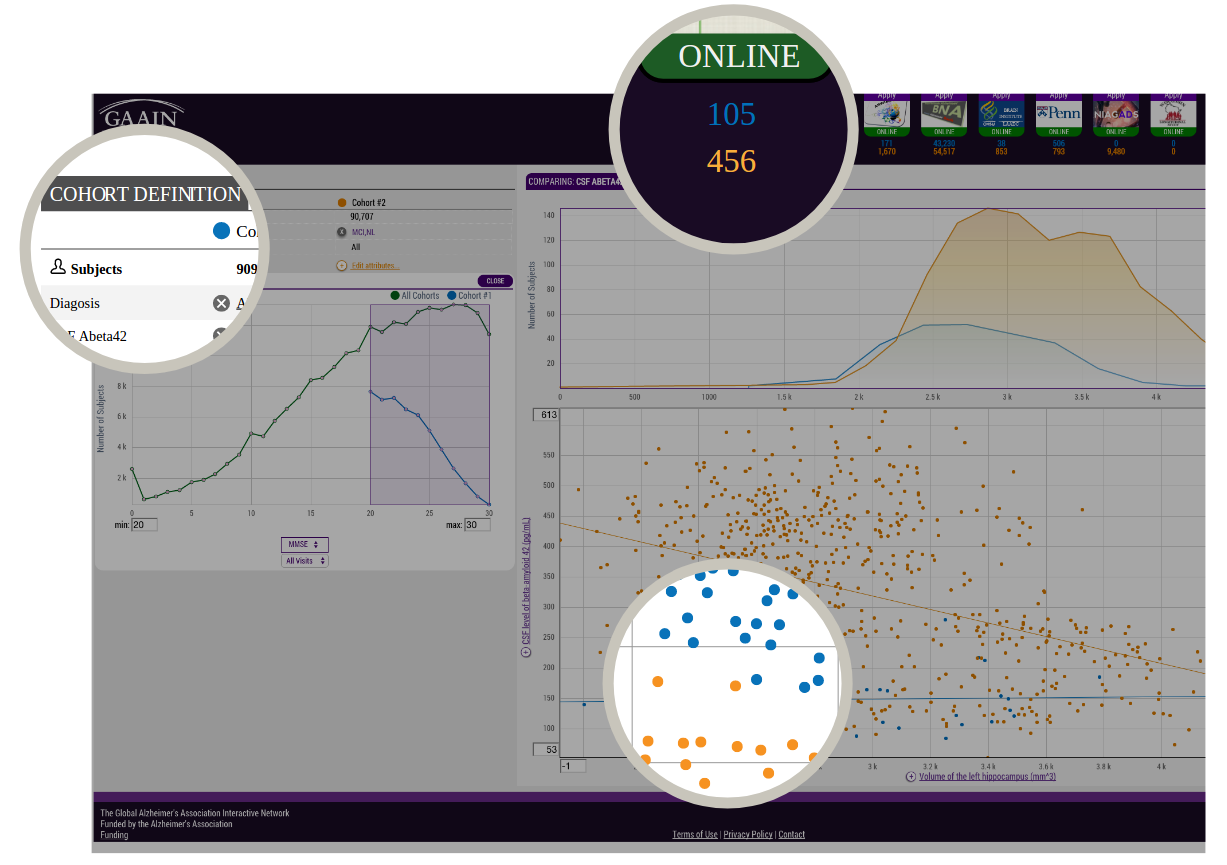
\includegraphics[height=4.5cm,right]{interrogator.png}   
\end{figure}

\end{frame}

% \begin{frame}
% \frametitle{European Medical Information Framework for Alzheimer’s disease (EMIF-AD})
% 
% \begin{itemize}
%  \item 
% \end{itemize}
% 
% 
% 
% \end{frame}

\fontsize{6pt}{7.2}\selectfont
\rowcolors{2}{gray!25}{white}

% \begin{frame}
% \frametitle{Validation methods for disease progression models}
% 
% \begin{tabular}{p{3.3cm} p{3.3cm} p{3.3cm}}
%  Method & Pros & Cons\\
%  \hline
%  AIC/BIC & no extra data required & \\
%  Staging consistency & &\\
%  Elapsed time prediction & &\\ 
%  Diagnosis prediction and differential diagnosis & & diagnosis not precise, required post-mortem confirmed data\\
%  Correlation of stages with clinical markers & & relationship not linear\\
%  Simulations & ground truth available & simulated data might not reflect actual data\\
%  Prediction of leave-out biomarkers & & \\
%  Resampling methods & can also be used to test accuracy of model parameters & computationally intensive\\
%  Reproducibility across models and datasets & & requires different datasets\\
% \end{tabular}
% 
% \end{frame}


 
\end{document}

